\documentclass[12pt,a4paper]{report}
\usepackage[utf8]{inputenc}
\usepackage[english,russian]{babel}
\usepackage{indentfirst}
\usepackage{pdfpages}
\usepackage{titlesec}
\usepackage{listings}
\usepackage{amsmath}

% Вставка картинки
\usepackage{graphicx}
\graphicspath{{schemes/}}
\DeclareGraphicsExtensions{.pdf,.png,.jpg}

\usepackage[14pt]{extsizes}

\newcommand{\hsp}{\hspace{20pt}}
\titleformat{\chapter}[hang]{\large\bfseries}{\thechapter{. }}{0pt}{\large\bfseries}
\titlelabel{hlabel-formati}
\titlespacing{\chapter}{42pt}{-20pt}{12pt}
\titleformat{\section}[hang]{\large\bfseries}{\thesection{. }}{0pt}{\large\bfseries}
\titlespacing{\section}{42pt}{12pt}{5pt plus 5pt}

% Отступ абзаца
\usepackage{indentfirst}
\setlength{\parindent}{1.5cm}

% Межстрочный интервал
\usepackage{setspace}
\onehalfspacing % интервал 1.5

\usepackage[left=3cm, right=1cm, top=2cm, bottom=2cm]{geometry}

\AtBeginDocument{%
	\renewcommand\contentsname{Содержание}
}

\usepackage[tableposition=top,singlelinecheck=false]{caption}

\begin{document}
% Титульник

\includepdf[pages=1]{titul.pdf}
% Оглавление
\tableofcontents\contentsname

\newpage
\chapter*{Введение}
\addcontentsline{toc}{chapter}{Введение}
В этой лабороторной работе мы рассматриваем вопрос, который часто
 возникает в программировании - перемещение элементов в порядке
 возрастания или убывания. Можно легко представить, как бы усложнило 
 жизнь пользование словарем, в котором слова расположены не в
 алфовитном порядке. Точно также, от порядка хранения элементов в памяти
 компьютера, зависит скорость выполнения и простота
  алгоритмов над этими элементами.

 Вот одни из наиболее важных областей применения сортировок:


 \begin{itemize} 
    \itemрешение задач групперирования, когда нужно собрать 
    вместе все элементы с одинаковыми значениями некоторого признака;
    \item поиск общих элементов в двух и более массивах; 
    если два и более массива рассортировать в одном и том же порядке,
    то можно найти одинаковые элементы за один последовательный просмотр
    без возвратов; 
    \item поиск информации по значениям ключей. 
  \end{itemize}

Цель данной лабораторной работы заключается в изучении алгоритмов 
сортировки массивов. Рассматриваются алгоритмы сортировки пузырьком,
вставками и Шейкер сортировка. Требуется расчитать и изучить трудоемкость
и затрачиваемое каждым алгоритмом время.

Выделим следующие задачи:

\begin{itemize}
	\item изучить работу алгоритмов сортировки;
	\item выполнить полную математическую оценку трудоемкости
	для алгоритмов сортировки с указанием лучшего и худшего
	случаев;
	\item реализовать три алгоритма сортировки;
	\item сравнить работу алгоритмов сортировок и сделать выводы.
\end{itemize}
 
\newpage
\chapter{Аналитическая часть}

В данном разделе будут рассмотрены алгоритмы сортировки пузырьком, вставками и шейкерная сортировка.
Также разобраны принципы работы этих алгоритмов.

\section{Сортировка пузырьком (Bubble sort)}

Сортировка пузырьком — это простейший и один из самых известных
 алгоритмов сортировки. Идея заключается в последовательном 
 сравнении значений соседних элементов. Если текущий элемент 
 больше следующего, меняем их местами. Алгоритм необходимо 
 повторять до тех пор, пока массив не будет отсортирован.

 Этот алгоритм считается учебным и почти не применяется на
  практике из-за низкой эффективности: он медленно работает 
  на тестах, в которых маленькие элементы (их называют 
  «черепахами») стоят в конце массива. Однако на нём основаны 
  многие другие методы, например, шейкерная сортировка и 
  сортировка расчёской.

\section{Сортировка вставками (Insertion sort)}

Сортировка вставками - алгоритм, при котором каждый последующий
 элемент массива сравнивается с предыдущими элементами 
 (отсортированными) и вставляется в нужную позицию.

Общая идея алгоритма:

\begin{enumerate}
    \item Сравниваем второй элемент с первым элементом массива и 
    при необходимости меняем их местами. Условно эти элементы 
    (первый и второй) будут являться отсортированным массивом,
     остальные элементы - неотсортированным.
    \item  Сравниваем следующий элемент из неотсортированного массива 
    с элементами отсортированного и вставляем в нужную позицию.
    \item Повторям шаг 2 до тех пор, пока в неотсортированном массиве 
    не останется элементов.
\end{enumerate}


\section{Cортировка перемешиванием (Shaker)}

Также известна как шейкерная или коктейльная сортировка.

Сортировка перемешиванием - это разновидность сортировки пузырьком.
 Отличие в том, что данная сортировка в рамках одной итерации 
 проходит по массиву в обоих направлениях (слева направо и справа
  налево), тогда как сортировка пузырьком - только в одном 
  направлении (слева направо).

Общая идея алгоритма:

\begin{enumerate}
    \item 
    Обход массива слева направо, аналогично пузырьковой
     - сравнение соседних элементов, меняя их местами, 
     если левое значение больше правого. В итоге наибольшее 
     число будет перемещено в конец массива.
    \item Обход массива в обратном направлении (справа налево), 
    начиная с элемента, который находится перед последним 
    отсортированным. На этом этапе элементы также сравниваются 
    между собой и меняются местами, чтобы наименьшее значение 
    всегда было слева. В итоге наименьшее число будет перемещено 
    в начало массива.
\end{enumerate}

\section*{Вывод}

Таким образом, были рассмотрены алгоритмы сортировки пузырьком, вставками и шейкерная сортировка.
Также разобраны принципы работы этих алгоритмов.

Входными данными реализуемого ПО являются:

\begin{itemize}
	\item размерность массива - целое число;
	\item целочисленный массив;
\end{itemize}

Выходными данными реализуемого ПО являеться результат алгоритмов сортировки т. е. отсортированный массив по возростанию.

Ограничением для реализуемого ПО является - размерность вводимого массива т. е. введеное число должно быть натуральным.
	

\newpage
\chapter{Конструкторская часть}

В данном разделе будут сформированы требования к программе и составлены схемы алгоритмов.
Также подсчитана трудоёмкость для каждого их алгоритмов.


\section{Схемы алгоритмов}

На рисунках 2.1 - 2.4 приведены схемы алгоритмов сортировки массива.

\begin{figure}[h!]
    \center{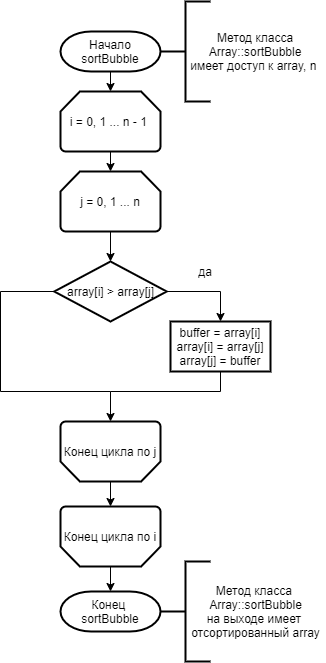
\includegraphics[scale=0.7]{bubbleSort}}
    \caption{Схема сортировки пузырьком}
    \label{fig:image}
\end{figure}

\begin{figure}[h!]
    \center{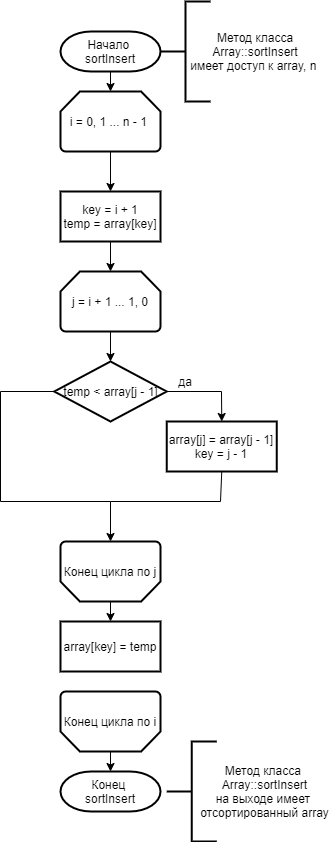
\includegraphics[scale=0.8]{insertSort}}
    \caption{Схема сортировки вставками}
    \label{fig:image}
\end{figure}

\begin{figure}[pt!]
	\center{\includegraphics[scale=0.8]{ShakerSort_1}}
	\caption{Схема сортировки перемешиванием}
	\label{fig:image}
\end{figure}

\begin{figure}[pt!]
	\center{\includegraphics[scale=0.8]{ShakerSort_2}}
	\caption{Схема сортировки перемешиванием}
	\label{fig:image}
\end{figure}

\section{Структура ПО}

На рисунке 2.5 представлена диограмма классов.

\section*{}
\begin{figure}[ht]
	\center{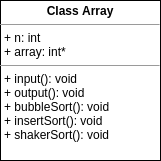
\includegraphics[scale=0.8]{structPO}}
	\caption{Диаграмма классов реализуемого ПО}
	%\label{fig:image}
\end{figure}

\section{Тестирование}

В рамках данной лабораторной работы были выделены следующие классы эквивалентности:
\begin{itemize}
	\item входными данными является отсортированный по возрастанию массив;
	\item входными данными является отсортированный по убыванию массив;
	\item входными данными является не сортированный массив;
\end{itemize}

Для проверки работы программы будет осуществлено тестирование согласно классам эквивалентности.

\newpage
\section{Подсчет трудоемкости алгоритмов}

Введем модель вычисления трудоемкости для оценки алгоритмов:

\begin{itemize}
    \item базовые операции стоимостью 1 -- $+, -, \cdot , /, =, ==, <=, >=, !=, +=, []$;
    \item оценка трудоёмкости цикла for от 0 до N с шагом 1 $F_{for} = 2 + N \cdot (2 + F_{body})$, где $F_{body}$ -- тело цикла;
    \item стоимость условного перехода примем за 0, стоимость вычисления условия остаётся. 
\end{itemize}

Оценим трудоёмкость алгоритмов сортировки массива по коду программы.

\textbf{Сортировка пузырьком} \\

Лучший случай -- $2 + 2 \cdot N + 3 \cdot N \cdot N$

Худший случай -- $2 + 2 \cdot N + 6 \cdot N \cdot N$ \\

\textbf{Сортировка вставками} \\

Лучший случай -- $2 + 9 \cdot N + 7/2 \cdot N \cdot N$

Худший случай -- $2 + 2 \cdot N + 11/2 \cdot N \cdot N$ \\

\textbf{Шейкерная сортировка} \\

Лучший случай -- $12 \cdot N \cdot N + 7 \cdot N + 5$

Худший случай -- $28 \cdot N \cdot N + 7 \cdot N + 5$

\section*{Вывод}

Таким образом, выше были сформированы требования к программе и составлены схемы алгоритмов.
Также подсчитана трудоёмкость для каждого их алгоритмов.

\newpage
\chapter{Технологическая часть} 


В данном разделе будут реализованы функции алгоритмов сортировки массивов на языке C++.

\section{Требования к программе}

Для дальнейшего использования программы необходимо обеспечить 
консольный ввод размера массива, далее пользователю предостовляется 
выбор, ввести массив вручную или сгенерировать. С полученным массивом
возможно произвести сортировку из предложенных(пузыркем, вставками и Шейкер).
Также необходимо реализовать функцию подсчета процессорного времени,
которое затрачивает функция.

\section{Выбор языка программирования}

В качестве языка программирования было решено выбрать C++, 
так как уже имеется опыт работы с библиотеками и инструментами
языка, которые позволяют реализовать и провести исследования над 
алгоритмами сортировки массивов.

\section{Сведенья о модулях программы}

Программа состоит из:

main.cpp -  главный файл программы, в котором распологается точка входа.

array.h - класс Array, который содежит алгоритмы сортировок

array.cpp - реализация методов класса Array

\section{Реализация алгоритмов}

В листингах 3.1 - 3.3 приведены реализации алгоритмов
сортировки массивов на ЯП C++.

\noindent\textrm{Листинг 3.1: реализация сортировки пузырьком}
\begin{lstlisting}[frame=single, numbers=left]
    void Array::sortBubble()
    {
        for (int i = 0; i < n; i++)
            for (int j = 0; j < n - 1; j++)
                if (array[j] > array[j + 1])
                    swap(array[j], array[j + 1]);
    }
\end{lstlisting}

\noindent\textrm{Листинг 3.2: реализация сортировки вставками}
\begin{lstlisting}[frame=single, numbers=left]
    void Array::sortInsert()
    {
        int key = 0;
        int temp = 0;
        for (int i = 0; i < n - 1; i++)
        {
            key = i + 1;
            temp = array[key];
            for (int j = i + 1; j > 0; j--)
                if (temp < array[j - 1])
                {
                    array[j] = array[j - 1];
                     key = j - 1;
                }
            array[key] = temp;
        }
    }
\end{lstlisting}

\noindent\textrm{Листинг 3.3: реализация сортировки перемешиванием}
\begin{lstlisting}[frame=single, numbers=left]
    void Array::sortShaker()
    {
        int left = 0;
        int right = n - 1;
        int flag = 1;
        while((left < right) && (flag > 0))
        {
            flag = 0;
            for (int i = left; i < right; i++)
                if (array[i] > array[i + 1])
                {
                    swap(array[i], array[i + 1]);
                    flag = 1;
                }
            right--;
            for (int i = right; i > left; i--)
                if (array[i - 1] > array[i])
                {
                    swap(array[i - 1], array[i]);
                    flag = 1;
                }
            left++;
        }
    }
\end{lstlisting}

\noindent\textrm{Листинг 3.4: реализация функции обмена значений переменных (swap)}
\begin{lstlisting}[frame=single, numbers=left]
	void Array::swap(int &a, int &b)
	{
		int value = a;
		a = b;
		b = value;
	}
\end{lstlisting}


%\section{Тестирование алгоритмов}

\section*{Вывод}

По итогу, были реализованы функции алгоритмов сортировки массивов на языке C++.

\newpage
\chapter{Исследовательская часть} 

В данном разделе сравним работу каждого алгоритма.

\section{Примеры работы}

\begin{figure}[ht]
	\center{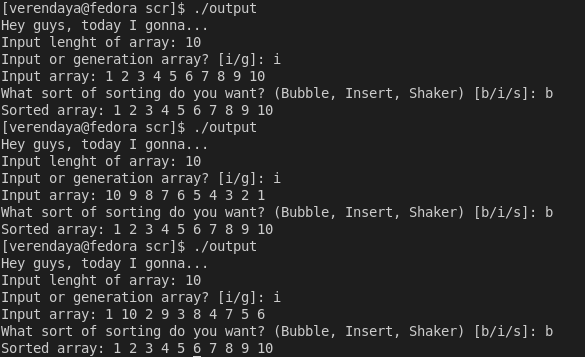
\includegraphics[scale=0.6]{BubbleData}}
	\caption{Пример работы алгоритма пузырьком(BubbleSort).}
	\label{fig:image}
\end{figure}

\begin{figure}[ht]
	\center{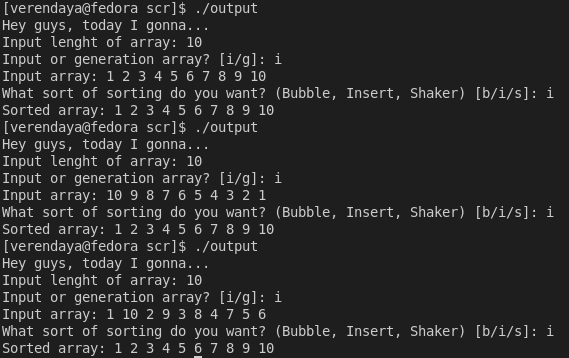
\includegraphics[scale=0.6]{InsertData}}
	\caption{Пример работы алгоритма вставками(InsertSort).}
	\label{fig:image}
\end{figure}


\begin{figure}[ht]
	\center{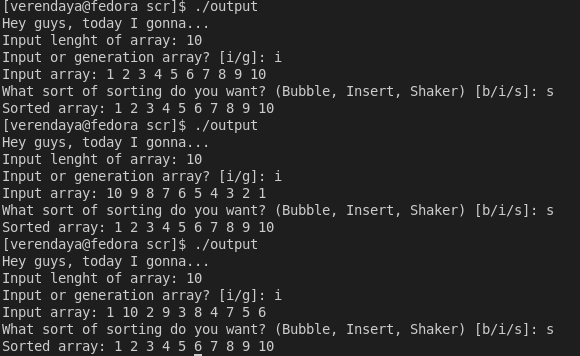
\includegraphics[scale=0.6]{ShakerData}}
	\caption{Пример работы алгоритма перемешиванием(ShakerSort).}
	\label{fig:image}
\end{figure}



\newpage
\section{Оценка затрачиваемого времени}

Далее будут приведены графики сравнения работы алгоритмов для каждого класса эквивалентности.

%\begin{figure}[ht]
%	\center{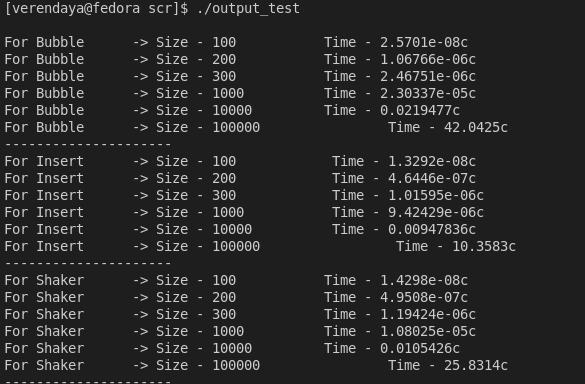
\includegraphics[scale=0.6]{testCPUTime}}
%	\caption{Таблица, содержащая временные характеристики алгоритмов сортировок.}
%	\label{fig:image}
%\end{figure}

\begin{figure}[ht!]
	\center{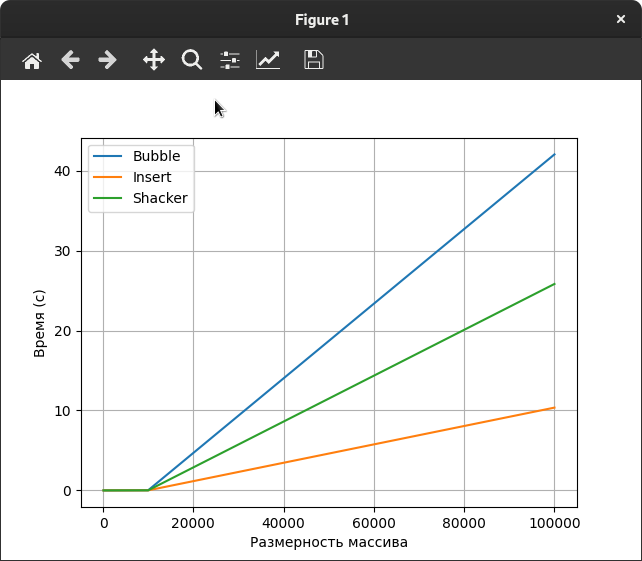
\includegraphics[scale=0.5]{random}}
	\caption{Сравнение работы алгоритмов на не отсортированных массивах.}
	\label{fig:image}
\end{figure}


\begin{figure}[ht!]
	\center{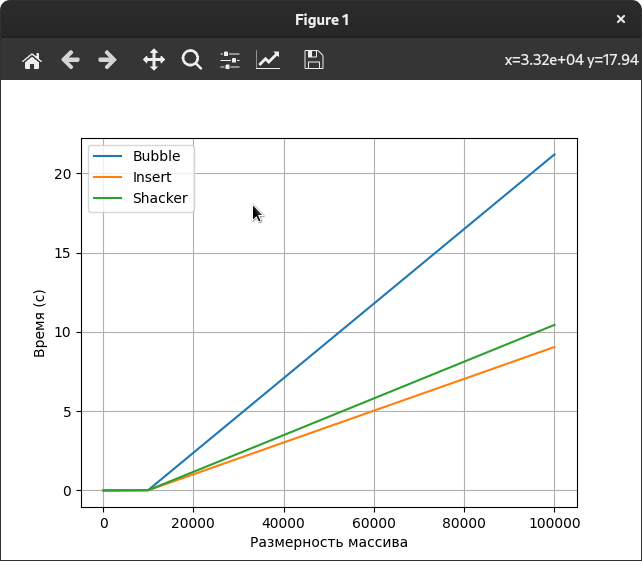
\includegraphics[scale=0.5]{sort}}
	\caption{Сравнение работы алгоритмов на отсортированных массивах по возростанию.}
	\label{fig:image}
\end{figure}


\begin{figure}[ht!]
	\center{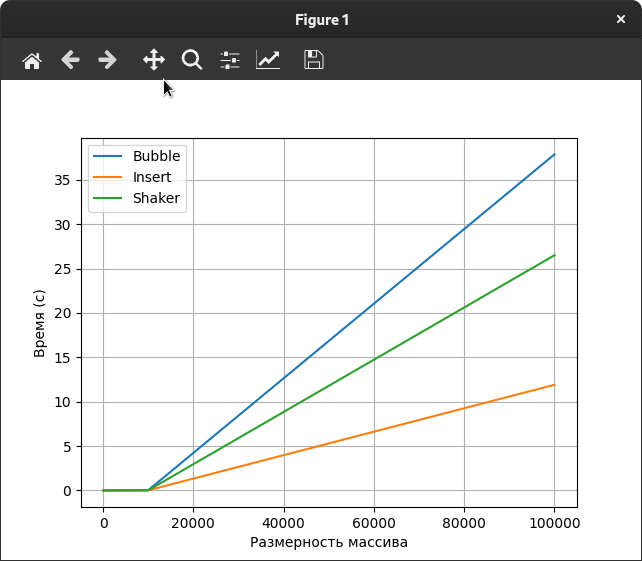
\includegraphics[scale=0.5]{unsort}}
	\caption{Сравнение работы алгоритмов на отсортированных массивах по убыванию.}
	\label{fig:image}
\end{figure}



\section*{Вывод}

Анализируя результаты замеров затрачиваемого времени можно сказать, что самым быстрым алгоритмом из представленных, при использовании 
случайного заполнения, оказался алгоритм сортировки вставками, а алгоритм сортировки пузырьком и шейкерная сортировка 
являются разновидностями пузырьковой сортировки.
Однако шейкерная сортировка работает в два раза быстрее пузырька.

\newpage
\chapter*{Заключение}
\addcontentsline{toc}{chapter}{Заключение}

В ходе работы были изучены алгоритмы сортировки массивов. 
Реализованы 3 алгоритма, приведен программный код реализации алгоритмов сортировки.
Была подсчитана трудоемкость каждого из алгоритмов, а также проведено сравнение алгоритмов по времени
 и трудоемкости. Показано, что наименее трудоемким и наименее затратным по времени алгоритмом является 
алгоритм сортировки вставками.\\

Цель работы достигнута, решены поставленные задачи.
Получены практические навыки реализации алгоритмов сортировки массивов, а также проведена 
исследовательская работа по вычислению трудоемкости алгоритмов и анализу их временных характеристик.


\newpage
\renewcommand\bibname{Список литературы}
\addcontentsline{toc}{chapter}{Список литературы}
\makeatletter % список литературы
\def\@biblabel#1{#1. }
\makeatother
\begin{thebibliography}{2}
    \bibitem{analyse_info} Дж. Макконнел. Анализ алгоритмов. Активный обучающий подход. -- М.: Техносфера, 2017. -- 267с.
    %\bibitem{} https://bimlibik.github.io/posts/sorting-algorithm/
    \bibitem{}Шагбазян, Д.В.     Алгоритмы  сортировки.  Анализ,  реализация,  применение: учебное  пособие  /  Д.В. Шагбазян,  А.А.  Штанюк,  Е.В.  Малкина. – Нижний Новгород: Нижегородский госуниверситет, 2019. – 42 с. 
    \bibitem{} Основы программирования на языках Си и C++ для начинающих[Электронный ресурс]. Режим доступа: http://cppstudio.com/ (дата обращения 10.10.2021)
    \bibitem{analyse_info}LINUX.ORG.RU - Русскоязычная информация о ОС Linux[Электронный ресурс] Режим доступа://www.linux.org.ru/(дата обращения 25.10.2021)
    \bibitem{analyse_info}Кнут Д. Э. Искусство программирования. Том 3. Сортировка и поиск = The Art of Computer Programming. Volume 3. Sorting and Searching / под ред. В. Т. Тертышного (гл. 5) и И. В. Красикова (гл. 6). — 2-е изд. — Москва: Вильямс, 2007. — Т. 3. — 832 с. — ISBN 5-8459-0082-1.
\end{thebibliography}

\end{document}
